%
% Documento: Desenvolvimento
%

\chapter{Desenvolvimento}

O desenvolvimento deste trabalho passou por quatro etapas principais: a seleção das técnicas a serem analisadas, a configuração do servidor de testes, a implementação dos testes e a execução dos testes. Neste capítulo estão descritos os detalhes dessas quatro etapas e as dificuldades encontradas em cada uma delas.

\section{Técnicas Escolhidas}
\label{tecnicasescolhidas}

Após análise das técnicas propostas por Steve Souders em seus livros, foi concluído que cinco técnicas poderiam sofrer alterações com a implantação do novo protocolo. São estas:

\begin{enumerate}
	\item Faça menos requisições HTTP
	\item Reduza o número de pesquisas DNS
	\item Evite redirecionamentos
	\item Lidando com \textit{scripts} assíncronos
	\item Quebrando domínios dominantes
\end{enumerate}

Das cinco técnicas listadas acima, apenas quatro puderam ser testadas. Isso porque a funcionalidade que melhorará o desempenho da técnica 4 ainda não foi implementada no servidor de teste escolhido. Mas, para complementar a análise da melhora de desempenho causada pelo HTTP/2, um quinto teste foi feito utilizando um \textit{template} de página \textit{web} e simplesmente o executando no HTTP/1.1 e depois no HTTP/2.

Para cada teste, foram criados projetos HTML separados. Dessa forma o comportamento de uma técnica não interfere na outra. Além disso, foram incluídos arquivos CSS e \textit{JavaScript} de maneira aleatória para a realização dos testes. Esses arquivos são de bibliotecas famosas e não foram alterados, apenas concatenados na realização de testes que necessitavam o uso dessa técnica. As bibliotecas escolhidas foram:

\begin{itemize}
	\item Animate CSS (\textit{https://daneden.github.io/animate.css/})
	\item Bootstrap (\textit{http://getbootstrap.com/})
	\item JQuery (\textit{https://jquery.com/})
	\item Font Awesome (\textit{https://fortawesome.github.io/Font-Awesome/})
	\item Full Calendar (\textit{http://fullcalendar.io/})
	\item Normalize (\textit{https://necolas.github.io/normalize.css/})
	\item Skeleton (\textit{http://getskeleton.com/})
	\item Angular JS (\textit{https://angularjs.org/})
	\item Backbone JS (\textit{http://backbonejs.org/})
	\item D3 (\textit{http://d3js.org/})
	\item Ember JS (\textit{http://emberjs.com/})
	\item High Charts (\textit{http://www.highcharts.com/})
	\item Moment JS (\textit{http://momentjs.com/})
	\item Require JS (\textit{http://requirejs.org/})
\end{itemize}

Com o intuito de estressar a conexão simulando melhor o número de requisições de um site real, nos quatro primeiros testes, foram inseridas na página 28 imagens de diferentes tamanhos e formatos. Essa imagens são aleatórias e nunca são alteradas.

A seguir encontram-se a explicações de cada teste e seus códigos-fontes podem ser encontrados anexados ao final deste trabalho.

\subsection{Faça menos requisições HTTP}
\label{facamenosrequisicoeshttp}

Para a realização deste teste, vários arquivos CSS e \textit{JavaScript} foram inseridos na página. Primeiramente, os arquivos são inseridos separadamente e depois são concatenados e inseridos de uma só vez. A soma dos tamanhos dos arquivos separados é 285kB maior do que a soma dos arquivos concatenados, 1.24 MB, isso ocorre por causa da remoção de espaços em branco.

O código para o teste com arquivos separados pode ser encontrado no \autoref{apend:codigo_facamenosrequisicoeshttp_sep} e o código para o teste com os arquivos concatenados no \autoref{apend:codigo_facamenosrequisicoeshttp_concat}.

\subsection{Reduza o número de pesquisas DNS}
\label{reduzaonumerodepesquisasdns}

Neste teste, os mesmos arquivos CSS e \textit{JavaScript} do teste \ref{facamenosrequisicoeshttp} foram utilizados mas, desta vez, ao invés de serem hospedados no mesmo servidor dos arquivos HTML, eles foram inseridos via CDN. Sendo assim, as páginas se diferem no número de CDNs utilizadas. Enquanto no código do \autoref{apend:codigo_reduzaonumerodepesquisasdns_mult} são utilizadas 4 CDNs diferentes, no código do \autoref{apend:codigo_reduzaonumerodepesquisasdns_unic} apenas uma é utilizada. Com isso, no primeiro teste, são feitas quatro consultas de DNS e, no segundo, apenas uma.

\subsection{Evite redirecionamentos}
\label{eviteredirecionamentos}

A realização deste teste não depende apenas da página \textit{web} utilizada, mas também de mudanças na configuração do servidor. Sendo assim, a página \textit{web} utilizada para o primeiro teste também foi reutilizada e foi feita uma mudança no arquivo de configuração do servidor. Essa mudança definia que caso uma requisição fosse recebida pelo servidor em uma determinada porta, ela deveria ser redirecionada para outra porta.

\subsection{Quebrando domínios dominantes}
\label{quebrandodominiosdominantes}

Enquanto que no teste da \autoref{reduzaonumerodepesquisasdns} o número de pesquisas de DNS vai de um extremo ao outro, passa de 4 para 1, neste teste as medições são repetidas para 2 e 3 DNS diferentes na página, com o intuito de se encontrar o número ideal de consultas de DNSs que diminui o tempo de pesquisas e aumenta o paralelismo das requisições. O código para esse teste encontra-se no \autoref{apend:quebrandodominiodominantes}.

\section{O servidor}
\label{oservidor}

Um servidor é um programa de computador que recebe requisições e envia respostas. Na \textit{Web}, o tipo mais comum de requisição e resposta são as requisições e respostas HTTP. Sendo assim, a função primária de um servidor \textit{web} é aguardar por requisições HTTP e servir páginas \textit{web}.

Para este trabalho, três servidores foram considerados. De acordo com a \citeonline{PopularidadeServidores}, os dois primeiros são os servidores \textit{web} mais populares do mundo atualmente, o Apache\footnote{http://www.apache.org/} e o Nginx\footnote{http://nginx.org/}. Mas, como esses servidores ainda não possuem versões oficiais estáveis que implementam o HTTP/2, um outro servidor, o \textit{nghttp2}, foi o servidor considerado para lidar com o novo protocolo.

\subsection{Apache}
\label{apache}

O servidor \textit{web} Apache foi lançado em 1995 por um grupo de entusiastas que procuravam uma maneira segura, eficiente e escalável de servir páginas \textit{web} para todos.  De acordo com a \citeonline{ApacheHTTPD}, o servidor Apache se tornou o mais popular do mundo em Abril de 1996 e nunca mais perdeu essa posição. Desde o início, o projeto se desenvolveu como uma iniciativa de código livre e assim se mantém até os dias atuais. As grandes vantagens do Apache são que ele pode ser executado em qualquer sistema operacional UNIX\footnote{Família de sistemas operacionais que é utilizado como base do Linux e do iOS. https://en.wikipedia.org/wiki/Unix} ou Windows NT\footnote{Família de sistemas operacionais produzidas pelas \textit{Microsoft}. https://en.wikipedia.org/wiki/Windows\_NT} e é simples de ser configurado.

\subsection{Nginx}
\label{nginx}

Assim como o Apache, o Nginx é um projeto de código livre de servidor HTTP. Começou a ser desenvolvido em 2002 e teve sua primeira versão pública lançada em 2004. A motivação para a criação do Nginx foi encontrar uma solução para o problema C10K\footnote{http://www.kegel.com/c10k.html}, que diz que um servidor \textit{web} deve suportar 10 mil conexões paralelas. Sendo assim, como explica \citeonline{Nginx}, o servidor foi construído com um arquitetura completamente assíncrona que beneficia de pequenos serviços de hospedagem a grandes sistemas de computação paralela.

\subsection{Nghttp2}
\label{nghttp2}

O \textit{nghttp2}, desenvolvido por \citeonline{nghttp}, é uma implementação em linguagem C do HTTP/2 e do protocolo de compressão HPACK. Essa implementação possui um cliente, um servidor, um \textit{proxy} e uma ferramenta de teste de carga para o servidor. Apesar do nome sugerir que existe alguma ligação entre o Nginx e o \textit{nghttp2}, não foi possível encontrar nada que relacione os dois servidores.

Apesar de os passos para a instalação do \textit{nghttp2} estarem documentados no site do projeto, algumas etapas importantes sobre instalação de dependências necessárias para fazer a aplicação funcionar corretamente não estão bem explicadas. Sendo assim, foram encontradas dificuldades no processo de instalação. Mas após superar essas dificuldades a aplicação foi configurada e foi possível confirmar seu funcionamento com a ajuda de um navegador com suporte a requisições e respostas HTTP/2. O processo de instalação está descrito no \autoref{apend:configurandonghttp2}.

\subsection{A escolha do servidor}
\label{aescolhadoservidor}

Para executar os testes propostos, foi necessário utilizar um servidor que suportasse tanto requisições HTTP/1.1 quanto HTTP/2. Como o HTTP/2 ainda é recente, encontrar um servidor com tal característica se mostrou um grande desafio.

Existem várias implementações do protocolo no mercado, cada uma com características diferentes e em estados diferentes de maturidade\footnote{Para obter mais informações sobre as diferentes implementações do HTTP/2 acesse o link a seguir. https://github.com/http2/http2-spec/wiki/Implementations}. Mas o problema é que a grande maioria dessas implementações são privadas e específicas para as empresas que as desenvolveram. Até o dia 1 de Agosto de 2015 (data quando os testes foram executados pela primeira vez) não existiam versões oficiais do protocolo para o Apache ou para o Nginx.

Apesar de não existir uma versão oficial do HTTP/2 para o Apache, existe um projeto de código aberto chamado \textit{mod\_h2}, desenvolvido por \citeonline{ModH2}, que se tornará a versão oficial do protocolo quando atingir um nível de maturidade e estabilidade considerado aceitável pela Apache Foundation. Como para o Nginx não existia ainda uma extensão que implementasse o novo protocolo dentro do servidor, o Apache seria a melhor escolha de servidor de teste.

As instruções para a instalação do mod\_h2 podem ser encontradas no site oficial do módulo e incluem:
\begin{enumerate}
	\item Baixar os arquivos do projeto
	\item Gerar arquivos de configuração e construção do módulo
	\item Compilar o módulo
	\item Mudar configurações do Apache para utilizar o novo módulo
	\item Ativar suporte ao novo protocolo
\end{enumerate}

Apesar da aparentemente simplicidade das etapas, após várias tentativas, não foi possível concluir a configuração do módulo. Os arquivos foram compilados e foi gerado o arquivo executável necessário para a utilização do mod\_h2. Sendo assim, o próximo passo seria configurar o servidor para utilizar o novo protocolo como preferencial nas requisições e respostas HTTP. Mas, apesar de seguir todas as instruções descritas no site do mod\_h2, não foi possível fazer com que o Apache executasse o HTTP/2. O processo final utilizado está descrito no \autoref{apend:tentativadeconfiguracaomodh2}.

Como a configuração do servidor Apache falhou, foi necessário encontrar uma solução alternativa para executar o protocolo.

\subsubsection{A primeira escolha do servidor}
\label{aprimeiraescolhadoservidor}

Apesar dos esforços para encontrar um servidor que suportasse a várias versões do protocolo HTTP, tal feito não foi possível. Sendo assim, ficou decido que seriam utilizados dois servidores diferentes para a realização dos testes, um para o HTTP/1.1 e outro para o HTTP/2.

Como o \textit{nghttp2} foi o único servidor com suporte ao HTTP/2 que a instalação foi feita com sucesso, ele foi escolhido como o servidor de teste para o novo protocolo. E por apresentar desempenho melhor do que o Apache, o Nginx foi escolhido como o servidor de teste para o HTTP/1.1.


\section{Execução dos testes}
\label{execuçãodostestes}

Os testes foram realizados em navegadores \textit{web}, o que torna o processo independente do sistema operacional. Mas o servidor foi configurado em uma máquina utilizando o sistema Ubuntu 14.04LTS, sendo assim, vale ressaltar, que os comandos descritos não vão necessariamente funcionar em sistemas operacionais diferentes do utilizado neste trabalho.

\subsection{Considerações iniciais}
\label{consideracoesiniciais}

O \textit{nghttp2} permite a escolha do uso de HTTP/2 de duas maneiras:
\begin{enumerate}
	\item Utilização do \textit{nghttpx} para a criação de um \textit{proxy} para servidor HTTP/1.1
	\item Utilização do servidor \textit{nghttpd}
\end{enumerate}

Utilizar a primeira opção significa que o navegador vai mandar uma requisição HTTP/2 para a porta que o \textit{proxy} está escutando. Essa requisição vai então ser traduzida pelo \textit{proxy}, que vai transforma-lá em uma requisição HTTP/1.1 e vai redireciona-lá para o servidor HTTP/1.1 que está escutando outra porta. O servidor HTTP/1.1 vai fazer todas as operações necessárias e vai retornar uma resposta HTTP/1.1 para o \textit{proxy}, que vai traduzi-la para o HTTP/2 e retorna-la para o navegador. Esse processo está ilustrado na \autoref{fig:http2diagram}.

\begin{figure}[!htb]
    \centering
    \caption{Diagrama de funcionamento de proxy HTTP/2.}
    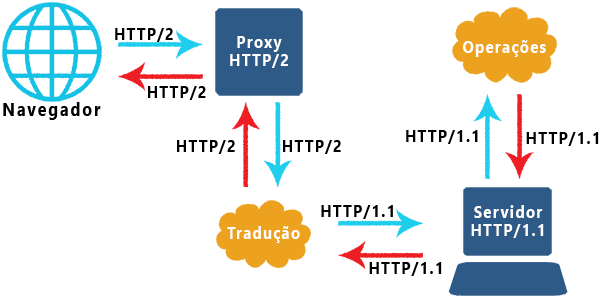
\includegraphics[width=0.8\textwidth]{./04-figuras/desenvolvimento/http2_proxy_diagram}
    \label{fig:http2diagram}
\end{figure}

Apesar de parecer muito custoso, a implementação desse \textit{proxy} já garante ao usuário uma melhora de desempenho de seu servidor, isso porque a comunicação HTTP/2 é mais rápida e melhora o paralelismos das conexões. Além disso, o \textit{proxy} ainda possibilita o uso de funcionalidades especificas do HTTP/2, como o \textit{Server Push}.

A segunda opção utiliza o \textit{nghttpd}, um servidor completo embutido dentro do \textit{nghttp2}, para fazer todo o trabalho. Dessa forma, o navegador se comunica com esse servidor que faz todo o processamento necessário e retorna a resposta para o navegador. Tudo isso utilizando o protocolo HTTP/2. A desvantagem desse método é que o \textit{nghttpd} não possui um arquivo de configuração, que é uma característica típica de servidores como o Apache e o Nginx e, por isso, ele acaba sendo limitado em alguns casos. Por exemplo, ainda não é possível utilizar o \textit{Server Push} com o \textit{nghttpd}, pois para configurar essa funcionalidade é necessário um arquivo de configuração.

Como os servidores de teste para cada protocolo já são diferentes, houve um grande esforço para deixar as configurações de ambiente restantes as mais similares possíveis, tentando assim evitar diferenças de desempenho provindas de outras configurações além da mudança de protocolo. Dessa forma, a escolha pela configuração utilizando o \textit{nghttpx} foi descartada. O redirecionamento via \textit{proxy} acrescentaria mais uma etapa no processo de comunicação cliente-servidor e, mesmo que se um \textit{proxy} fosse configurado para o servidor HTTP/1.1, ainda assim existe a etapa de tradução que não teria como ser simulada. Com isso, a configuração escolhida foi o uso do \textit{nghttpd}.

Como dito anteriormente, apesar de inicialmente o HTTP/2 ter sido desenvolvido para funcionar apenas sob o protocolo TLS para melhorar a segurança da \textit{Web}, essa proposta não foi aprovada e o HTTP/2 pode ser executado tanto com certificados de segurança como sem. A proposta inicial era executar os testes nos dois ambientes, HTTP e HTTPS, contudo o \textit{nghttpd} não funcionou corretamente quando foi executado sem um certificado de segurança, por isso, os testes foram feitos apenas com o protocolo HTTPS. Esse tipo de falha no servidor, embora seja um problema para aplicações que querem utilizar do novo protocolo, são esperadas, pela tecnologia ser ainda muito nova e não houve tempo ábil para corrigir todos os defeitos.

\subsection{Utilizando o \textit{nghttpd}}
\label{utilizandoonghttpd}

Para utilizar o \textit{nghttpd} foi necessária uma porta na máquina onde o servidor foi instalado para o cliente poder acessar o servidor \textit{web}, um arquivo de certificado digital e uma chave para tal certificado. Então, tendo o \textit{nghttp2} instalado, basta executar o seguinte comando:

\textbf{sudo nghttpd 83 /etc/apache2/ssl/dreamtech.key /etc/apache2/ssl/dreamtech.crt -d/var/www/html/tcc -v}

\begin{itemize}
	\item 83 define qual porta será escutada pelo servidor
	\item /etc/apache2/ssl/dreamtech.key é o caminho para o arquivo de chave do certificado digital
	\item /etc/apache2/ssl/dreamtech.crt é o caminho para o certificado digital
	\item -d define que uma pasta diferente da atual será servido pelo servidor
	\item /var/www/html/tcc é o caminho da pasta que será servida
	\item -v define que o servidor deverá exibir (verbalizar) as operações que está executando
\end{itemize}

Com isso o servidor para o protocolo HTTP/2 já está funcionando, apontando para a pasta /var/www/html/tcc e já pode ser acessado pela porta 83.

\subsection{A primeira execução dos testes}
\label{aprimeiraexecucaodostestes}

Para iniciar os testes foi necessário garantir que os navegadores escolhidos estavam com a opção de realizar requisições HTTP/2 habilitada. Enquanto que nas versões mais atuais do Google Chrome essa opção já vem habilitada por padrão e não existe mais uma forma de desabilita-la, no Mozilla Firefox foi necessário seguir o procedimento descrito a seguir para garantir que o navegador fizesse as requisições com o novo protocolo.

\begin{enumerate}
	\item Abra navegador
	\item Digite \textit{about:config} na barra de navegação
	\item Confirme que deseja alterar as configurações do seu navegador
	\item Na barra de pesquisa, procure por \textit{network.http.spdy.enabled.http2draft}
	\item Clique duas vezes na preferência e confirma que seu resultado foi alterado para verdadeiro
	\item Na barra de pesquisa, procure por \textit{security.ssl.enable\_alpn}
	\item Clique duas vezes na preferência e confirma que seu resultado foi alterado para verdadeiro	
\end{enumerate}

Por fim, para garantir que os navegadores estavam fazendo requisições HTTP/2, bastou iniciar o servidor \textit{nghttpd} e utilizar as ferramentas de desenvolvedor de cada navegador.

\begin{figure}[!htb]
    \centering
    \caption{Ferramentas do desenvolvedor do Google Chrome mostrando protocolo usado na requisição.}
    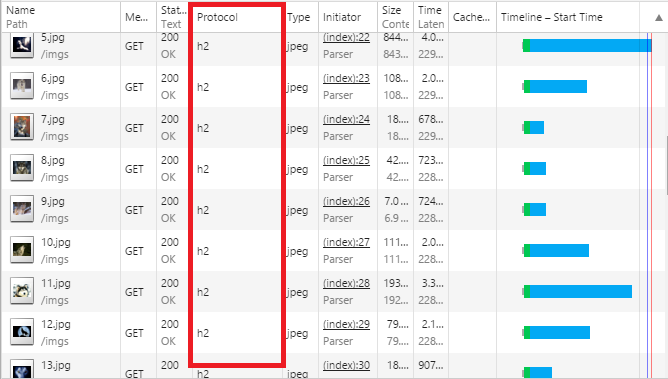
\includegraphics[width=1.0\textwidth]{./04-figuras/desenvolvimento/http2_chrome}
\end{figure}

\begin{figure}[!htb]
    \centering
    \caption{Ferramentas do desenvolvedor do Mozilla Firefox mostrando protocolo usado na requisição.}
    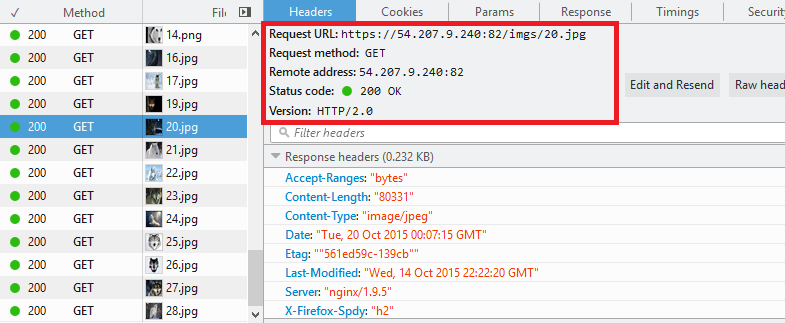
\includegraphics[width=1.0\textwidth]{./04-figuras/desenvolvimento/http2_firefox}
\end{figure}

Esse processo garantiu que o servidor e os navegadores funcionam, pois ambos podem se comunicar utilizando o protocolo HTTP/2. Sendo assim, pôde-se dar início ao processo de realização dos testes.

Como o servidor \textit{nghttpd} não possui um arquivo de configuração, foi necessário colocar cada caso de teste em pastas diferentes e, quando um caso novo fosse ser testado, o servidor tinha de ser reiniciado e apontado para outra pasta.

Para cada técnica de otimização escolhida, a página foi carregada 25 vezes utilizando o protocolo HTTP/1.1 no servidor \textit{Nginx} e 25 vezes utilizando o protocolo HTTP/2 no servidor \textit{nghttpd}. Os tempos de carregamentos das páginas foram registrados e foram calculadas as médias e o desvio padrão para cada técnica de otimização.

\subsection{Problemas nos resultados}
\label{problemasnosresultados}

Após a execução dos testes, percebeu-se que os resultados obtidos não foram os esperados. O HTTP/2 estava tendo resultados piores do que o HTTP/1.1 para todos os cenários de teste e as técnicas que não eram esperadas que funcionassem no novo protocolo, continuavam gerando tempos de carregamento diferentes quando aplicadas. Por esse motivo e levando em conta que o HTTP/2 é uma tecnologia muito nova e que suas implementações estão evoluindo de maneira acelerada, após a conclusão de que os resultados obtidos com o \textit{nghttp2} não eram satisfatórios, foi feita uma nova procura por servidores \textit{web} com suporte à nova versão do protocolo HTTP.

\section{A escolha final do servidor}
\label{aescolhafinaldoservidor}


No dia 22 de Setembro, foi lançada uma nova versão não estável do Nginx que possui suporte às duas versões do protocolo HTTP, sendo que o suporte ao HTTP/2 funciona apenas para conexões seguras, ou seja, utilizando o protocolo de segurança SSL. Até o momento, a versão do servidor utilizada para a realização dos testes em HTTP/1.1 era a versão estável 1.6.2, a nova versão com suporte ao HTTP/2 é a 1.9.5. Dessa forma ficou decidido que o essa nova versão seria utilizada para os testes dos dois protocolos.

Para instalar a versão 1.9.5 do Nginx foi necessário remover por completo a versão antiga, inserir o repositório de arquivos nas configurações do sistema operacional e instalar novamente o servidor. A seguir encontra-se o passo-a-passo dessa instalação.

\begin{enumerate}
	\item Remova a versão antiga do servidor: \textit{sudo apt-get purge nginx nginx-common}
	\item Adicione o novo repositório às configurações do sistema:
		\begin{center}
			\textit{sudo nano /etc/apt/source.list}
			Adicione as duas linhas abaixo ao final do arquivo
			\textit{deb http://nginx.org/packages/mainline/ubuntu/ trusty nginx}
			\textit{deb-src http://nginx.org/packages/mainline/ubuntu/ trusty nginx}
		\end{center}
	\item Atualize seu repositório: \textit{sudo apt-get update}
	\item Limpe a \textit{cache} do serviço de instalação e instale a nova versão do servidor: \textit{sudo apt-get clean \&\& sudo apt-get install nginx}
	\item Verifique a versão instalada: \textit{nginx --v}
\end{enumerate}

Após instalada a nova versão do Nginx, foi necessário configurar o servidor para que ele aceitasse as duas versões do protocolo HTTP. Para isso, é feita a edição do arquivo padrão de configuração do Nginx, o \textit{conf.d}, que se encontra no diretório de instalação do servidor. As seguintes configurações devem estar presentes nesse arquivo para que ele aceite o HTTP/1.1 na porta 81 e o HTTP/2 na porta 82.

\begin{center}
server {
    listen 81 ssl default\_server;

    ssl\_certificate    server.crt;
    ssl\_certificate\_key server.key;
    ...
}

server {
    listen 82 ssl http2 default\_server;

    ssl\_certificate    server.crt;
    ssl\_certificate\_key server.key;
    ...
}
\end{center}

Dessa forma, bastou seguir o mesmo processo utilizado para confirmar o funcionamento do \textit{nghttp2} e, com a ajuda de um navegador \textit{web} com suporte ao HTTP/2, confirmar que as requisições estão sendo aceitas utilizando o HTTP/1.1 na porta 81 e o HTTP/2 na porta 82, e estão sendo servidas com respostas na versão correta do protocolo.

Então os testes foram repetidos na nova configuração do servidor seguindo exatamente o mesmo processo descrito anteriormente e mais uma vez os resultados do tempo de carregamento de cada página de teste foi registrado para análise.